\section{Results and sensitivity analysis}\label{results}
This section presents the most relevant quantitative results of the proposed case study. Section \ref{res:district_heating} elaborates on the district heating option in the \textit{Directed Transition} scenario. Section \ref{res:heat_pump} focuses on the implementation of a heat pump system in the \textit{Societal Commitment} scenario where the model indicates feasible solutions for a retrofitted building with a lower heat demand only (compared with the default settings). A comparison of the results of the district heating and heat pump-based heat supply in the different scenarios quantified in this work is conducted in Section \ref{res:overview}. Finally, Section \ref{res:co2_shares} presents the results in case of varying CO\textsubscript{2} pricing cost allocation between the property owner and the tenants. 

\subsection{District heating in the Directed Transition scenario}\label{res:district_heating}
This section presents the results of the district heating implementation in the \textit{Directed Transition} scenario in detail. Figure \ref{fig:dt+dh} shows the net present value of cash flows in general, and revenues in particular, of the property owner and a single tenant within the time horizon of 2025-2040. Figure \ref{fig:dt+dh} (top left) presents the different items of the property owner consisting of the overnight investment costs\deleted{ (light blue)}, investment grant\deleted{ (blue)}, and rent-related revenues\deleted{ (yellow)}. Note that the latter represent the additional rent-related revenues due to the newly installed sustainable heating system. Figure \ref{fig:dt+dh} (bottom left) shows the development of the property owner's net present value of their cashflow over time. Thereby, it is shown that the investment pays off for the property owner by zero in 2040. The two Figures \ref{fig:dt+dh} (top right, bottom right) illustrate the corresponding tenant's cash flow items (top) and total net present value (bottom) until 2040. 

\begin{figure}[h]
	\centering
	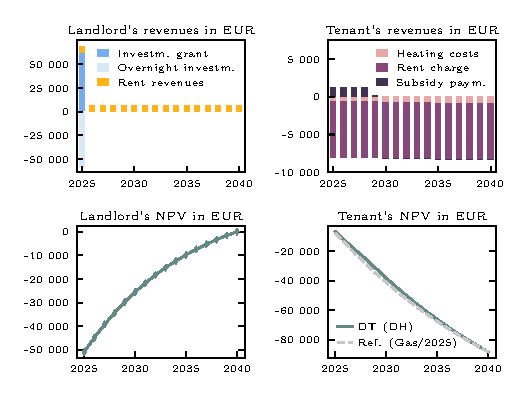
\includegraphics[width=0.9\linewidth]{figures/4_Results/fig_DT_DH/detail.eps}
	\caption{Development of the property owner's and tenant's economic viability of the district heating option in the \textit{Directed Transition} scenario. Top left: property owner's cash flows, bottom left: property owner's net present value, top right: tenant's cash flows, bottom right: tenant's net present value}
	\label{fig:dt+dh}
\end{figure}

 The tenant receives subsidy payments from the governance between 2025 and 2030. Thus, the tenant's net present value in 2040 matches with the value as in the reference case. The reference case considers constant remaining rent and heat-related costs for the tenant based on the initial rent, gas-based heat system parameters, and CO\textsubscript{2} prices as of 2025. In the years 2025-2029, the subsidy payments exceed the heating costs of the tenant. Note that the tenant already pays a higher rent charge to the property owner within the same period (see the yellow bars in Figure \ref{fig:dt+dh} top left). Most importantly, the tenant's reference net present value ("Ref. (Gas/2025)"; gray dashed line in the Figure \ref{fig:dt+dh} bottom right) shows a crucial aspect of the results and assumptions of the analysis which requires an explanation. Since "Ref. (Gas/2025)" is used as the initial tenant's spendings, the results also take into account the total opportunity costs (i.e., those costs that would be incurred by sticking to the initial gas-based heating system for the tenant due to a rising CO\textsubscript{2} price). Note that the openENTRANCE decarbonization scenarios used in this work do consider both a significant increase of the CO\textsubscript{2} price and a decrease of the specific emissions of the district heating and electricity fueling mix. The quantitative results indicate that the heating system change in this scenario is achieved with manageable total governance subsidies. However, a detailed discussion of the allocation of CO\textsubscript{2} price-related opportunity costs is conducted in Section \ref{res:co2_shares}.

\subsection{Heat pump and building stock quality in the Societal Commitment scenario}\label{res:heat_pump}
Interestingly, the model indicates for the heat pump implementation in the \textit{Societal Commitment} scenario an infeasible solution. The reason for that is, among others (investment costs of the air-sourced heat pump and the electricity price), the high heating demand used in the default input settings\footnote{\added{The high electricity demand resulting from the low COP and related increasing electricity costs need high subsidy payments for the tenants in this case. Against the background of comparable low investment costs of the property owner, Equation \ref{c:final} cannot be satisfied.}}. Therefore, in the following the focus is put on the impact of different building renovation levels, the associated heating demand decrease, and finally the impact on the feasibility of the model.\vspace{0.5cm} 

Figure \ref{fig:retrofitting} shows the results of the heat pump implementation in the \textit{Societal Commitment} scenario for four different building qualities (and thus heat demand levels) in detail. Since the initial setting of the default building in terms of total and peak heat demand leads to the infeasibility of the model, the following three additional renovation levels are studied: \SI{10}{\%}, \SI{20}{\%}, and \SI{30}{\%} reduction of both the total and peak heat demands. In Figure \ref{fig:retrofitting} (top left), the corresponding settings of the specific heat load (describing building quality) are indicated. In case of a \SI{10}{\%} reduction of the heat demand, the property owner receives a significant investment grant equivalent to \SI{29}{\%} of the property owner's total overnight investment costs of the building retrofitting measures (Fig. \ref{fig:retrofitting} top right). The associated tenant's subsidy payment takes place between 2025 and 2030 with a maximum of \SI{2~040}{EUR \per year} (Fig. \ref{fig:retrofitting} bottom left). The rent charge adjustment and related revenues remain almost constant during the period (Fig. \ref{fig:retrofitting} bottom right). In case of a \SI{20}{\%} reduction of the heat demand, the property owner receives only a small investment grant related to the total overnight investment costs (\SI{2}{\%}). The tenant's subsidy payment takes place between 2025 and 2032 with a maximum of \SI{2~556}{EUR \per year}. The property owner's rent-related revenues increase until 2031 and then remain constant. In case of a \SI{30}{\%} reduction of the heat demand, the property owner receives as before a small investment grant (\SI{3}{\%}). Instead, the property owner makes significant rent-related revenues (the highest among the three renovation levels). The tenant gets subsidy payments in most years, excluding 2026 and 2028 to 2030 (mainly as a result of the matching of the CO\textsubscript{2} price and the specific CO\textsubscript{2} emissions of the fueling energy mix). The maximum is \SI{2~796}{EUR \per year} in 2040. The lower heat energy-related costs as a result of the building renovation lead to higher rent charge payments. Hence, smaller investment grants supporting the property owner are sufficient. 

\begin{figure}[h]
	\centering
	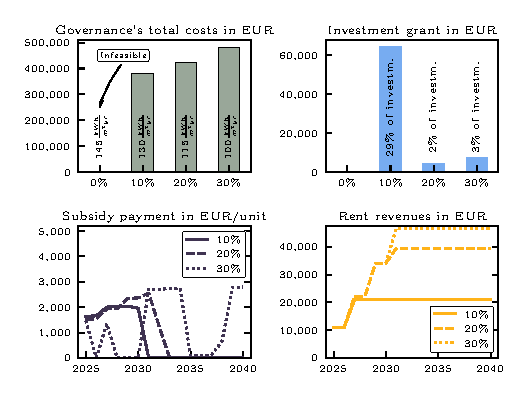
\includegraphics[width=0.95\linewidth]{figures/4_Results/fig_retrofitting/retrofitting.eps}
	\caption{Comparison of the heat pump option in the \textit{Societal Commitment} (SC) scenario for different renovation levels. Top left: governance's objective value, top right: property owner's investment grant, bottom left: tenant's subsidy payment per unit, bottom right: property owner's rent-related revenues in total}
	\label{fig:retrofitting}
\end{figure}

\subsection{Governance's total subsidies in the different scenarios}\label{res:overview}
In this section, a comparison of the governance's total subsidies for district heating (DH) or heat pump (HP) implementation in the different scenarios is conducted. Table \ref{tab:objective} and Figure \ref{fig:npv_comparison} present the result of this comparison. 

\definecolor{Gray}{gray}{0.95}
\begin{table}[h]
	\centering
	\scalebox{0.8}{
		\renewcommand{\arraystretch}{1.35}
		\begin{tabular}{lcccccc}
			\toprule 
			& \multicolumn{3}{c}{District heating (DH)} & \multicolumn{3}{c}{Heat pump (HP)}\\
			\cmidrule(lr){2-4}\cmidrule(lr){5-7}
			\multirow{2}{*}{Governance's total financial support}& DT & GD & LD & SC & GD& LD\\
			\cmidrule(lr){2-2}\cmidrule(lr){3-3}\cmidrule(lr){4-4}\cmidrule(lr){5-5}\cmidrule(lr){6-6}\cmidrule(lr){7-7}
			& (\SI{1.5}{\degreeCelsius}) & (\SI{2.0}{\degreeCelsius}) & (-) & (\SI{1.5}{\degreeCelsius}) &  (\SI{2.0}{\degreeCelsius}) & (-)\\
			\hline
			Absolute in thous. \SI{}{EUR} & \SI{211.4}{} & \SI{195.5}{} & \cellcolor{Gray}\SI{190.1}{} & \multirow{4}{*}{{\rotatebox[origin=c]{90}{\parbox{2cm}{\centering \textit{infeasible}}}}} & \multirow{4}{*}{{\rotatebox[origin=c]{90}{\parbox{2cm}{\centering \textit{infeasible}}}}} & \SI{351.5}{}\\
			Rel. change in \% of LD (DH) & \SI{11.2}{} & \SI{2.8}{} & - &  & & \SI{82.6}{}\\
			\added{CO\textsubscript{2} tax revenues in thous. EUR} & \added{66.6} & \added{38.9} & \added{25.7} & & & \added{10.3}\\
			\added{Public financial deficit in thous. EUR} & \added{144.8} & \added{156.6} & \added{164.4} & &  & \added{341.2}\\
			\bottomrule
	\end{tabular}}
	\caption{Comparison of governance's total financial support for the different heating system alternatives and scenarios \added{(incl. CO\textsubscript{2} tax revenues and public financial deficit)}}
	\label{tab:objective}
\end{table}

In summary, the following interesting observations are made:

\begin{itemize}
	\item The total subsidies across the three district heating cases are relatively stable and are within \SI{11.2}{\%}.
	\item The heat pump implementation in the two decarbonization scenarios \textit{Societal Commitment} and \textit{Gradual Development} is infeasible for the default setting of the building quality (see discussion already in Section \ref{res:heat_pump}).
	\item Only the low CO\textsubscript{2} price development scenario provides a solution for the heat pump but with a significantly higher subsidy +\SI{82.6}{\%} compared with the lowest subsidy scenario.
	\item \added{The public financial deficit (governance's total financial support minus CO\textsubscript{2} tax revenues) is the lowest (144.8 thous. EUR) in the \textit{Directed Transition} scenario.}
\end{itemize}

\begin{figure}[h]
	\centering
	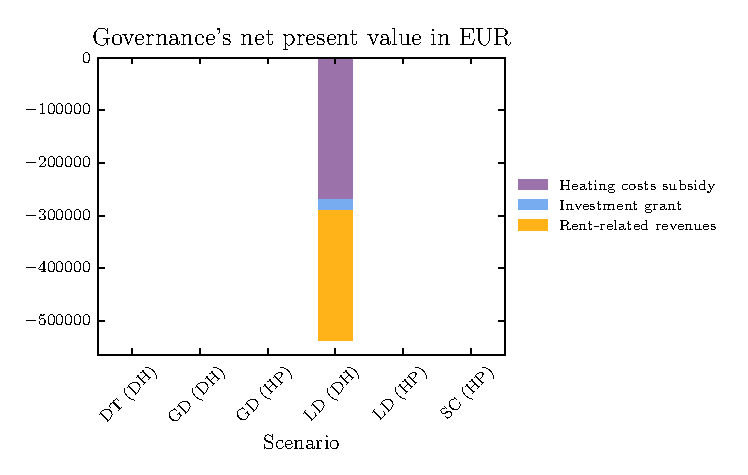
\includegraphics[width=0.7\linewidth]{figures/4_Results/fig_npv_comparison/net_present_value.eps}
	\caption{Comparison of governance's total financial support for the property owner and the tenants for the district heating (DH) and heat pump (HP) implementations in the different scenarios}
	\label{fig:npv_comparison}
\end{figure}

When comparing Table \ref{tab:objective} and Figure \ref{fig:npv_comparison}, it is important to note that the property owner's rent-related revenues (orange bar) are an "implicit" subsidy. Hence, the governance's total financial support is equal to the sum of the tenants' heating costs subsidy (purple bar) and the property owner's investment grant (blue bar). 

\subsection{Allocation of CO\textsubscript{2} pricing related costs between the governance, property owner, and tenant}\label{res:co2_shares}
This section examines the impact of the costs of inaction (i.e., sticking to the initial gas-based heating system) on the governance's total financial support. In detail, this means that the CO\textsubscript{2} costs (i.e., opportunity costs) to be expected due to increasing CO\textsubscript{2} prices have to be allocated to the different parties/agents (or a single one): governance, property owner, and tenant. \added{Table \ref{tab:co2allocation} shows the objective value (absolute value and relative change in \% from GD (DH)) for different allocations of opportunity costs.} Exemplarily, "Equally" (first row in Table \ref{tab:co2allocation}) takes into account that the CO\textsubscript{2} costs are shared equally among the governance, property owner, and tenants. Each of them bear one third of the costs. Note that the scenario setups from Section \ref{sec:scenarios} \added{(i.e., GD (DH))} considered so far that the total costs of inaction are covered by the governance (see Equations \ref{c:ten2} and \ref{c:ten4}). The mathematical formulation of the modifications here in this section can be found in \ref{app:varying}. Most importantly, the highest total subsidy reduction is obtained \replaced{when}{in "Case C" where} the property owner has to cover the costs of inaction (-\SI{49}{\%} compared with the reference value). The second highest reduction is \replaced{achieved when}{in "Case B". In this case,} the opportunity costs are shared equally within the building among the property owner and tenants (-\SI{34}{\%}). \replaced{Equally allocated opportunity costs}{"Case A"} reduce the total subsidy by \SI{25}{\%}.  It is evident that an even allocation between the governance and the tenants (\replaced{fourth row in Table \ref{tab:co2allocation}}{"Case D"}) hardly leads to a reduction of the objective value. The main reason for this is the financial support of the property owner, which is necessary to create an investment incentive, and the fact that the financial support between the property owner and tenants necessarily has the same net present value.\vspace{0.5cm}

Building upon, Figure \ref{fig:feasible} shows the objective value for the varying property owner's interest rates. The varying property owner's interest rates have two important impacts. First, a decreasing interest rate reduces the objective value as revenues are discounted less (see Fig. \ref{fig:feasible} for a fixed property owner's share in costs of inaction, e.g., $0.2$). Second, as the interest rate decreases, a feasibility limit becomes apparent. This means that the feasible maximum of the property owner's share in costs of inaction depends on the property owner's interest rate $i_l$ (e.g., \SI{100}{\%} for $i_l=\SI{10}{\%}$, \SI{70}{\%} for $i_l=\SI{5}{\%}$ and \SI{60}{\%} for $i_l=\SI{3}{\%}$). Two interesting energy policy implications can be derived from the results here:
\begin{itemize}
	\item In case the property owner is very much profit-oriented (e.g., interest rate of $\SI{10}{\%}$) and the governance's total subsidy payments are to be kept as low as possible, complete allocation of the CO\textsubscript{2}-related opportunity costs to the property owner results in a cost-optimal strategy.
	\item In contrast, in case the property owner rather serves a public-benefit purpose (e.g., interest rate of $\SI{3}{\%}$), the CO\textsubscript{2}-related opportunity costs allocation among governance, property owner, and tenants is an adequate strategy.
\end{itemize}

\definecolor{Gray}{gray}{0.95}
\begin{sidewaystable}
	\centering
	\setlength{\extrarowheight}{.5em}
	\resizebox{1\textwidth}{!}{
		\begin{tabular}{lccccc}
			\toprule
			& \multicolumn{3}{c}{Rel. allocation of opportunity costs} & \multicolumn{2}{c}{Objective value}\\\cmidrule(lr){2-4}\cmidrule(lr){5-6}
			Brief summary & Governance & Property owner & Tenant & Absolute in EUR & Rel. change in \% from GD (DH)\\\hline
			Equally & $\frac{1}{3}$ &  $\frac{1}{3}$ &  $\frac{1}{3}$ & 146.6 & -25\%\\
			Property owner \& tenant & 0 & $\frac{1}{2}$ &  $\frac{1}{2}$ & 129.0 & -34\%\\
			Property owner & 0 & $1$ &  0 & 99.7 & -49\%\\
			Governance \& tenant & $\frac{1}{2}$ & 0 &  $\frac{1}{2}$ & 183.8 & -6\%\\\hline
			\cellcolor{Gray} GD (DH) from Sec. \ref{sec:scenarios} (Governance)& \cellcolor{Gray}$1$ & \cellcolor{Gray}0 & \cellcolor{Gray}0 & \cellcolor{Gray}195.5 & \cellcolor{Gray}-\\
			\bottomrule
	\end{tabular}}
	\caption{\added{Comparison of objective value (absolute and in \%) for varying allocations of CO\textsubscript{2}-related opportunity costs. As reference serves the \textit{Gradual Development} scenario with district heating (GD (DH)) from Section \ref{sec:scenarios} where the total opportunity costs are allocated to the governance.}}
	\label{tab:co2allocation}
\end{sidewaystable}

\begin{figure}[h]
	\centering
	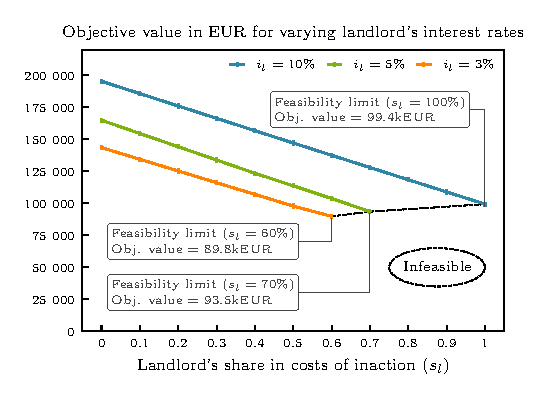
\includegraphics[width=0.85\linewidth]{figures/4_Results/fig_feasible/feasible.eps}
	\caption{Comparison of the objective value for varying property owner's interest rates and share in costs of inaction}
	\label{fig:feasible}
\end{figure}




